	\documentclass[25pt, a0paper, portrait]{tikzposter}
	
	\usepackage[utf8]{inputenc}
	\usepackage[T5]{fontenc}
	\usepackage[vietnamese]{babel}
	\usepackage{mathptmx}
	\renewcommand{\familydefault}{\rmdefault} % Fix font shape error by forcing serif as default
	\usepackage{amsmath,amssymb}
	\usepackage{graphicx}
	\usepackage{tabularx}
	\usepackage{xcolor, float, booktabs, colortbl}
	\usepackage{tikz}
	\usepackage{pgfplots}
	\pgfplotsset{compat=1.18}
	\usepackage{enumitem}
	\usepackage{algorithm}
	\usepackage{algpseudocode}
	% ================= MÀU SẮC & CHỦ ĐỀ CHUẨN TÍNH HỌC THUẬT (ĐÃ TINH CHỈNH) =================
	\usetheme{Envelope} 
	\usecolorstyle{Default}
	
	% 1. Định nghĩa lại bảng màu: Thêm điểm nhấn và chiều sâu
	\definecolor{PhenikaaBlue}{HTML}{0A3B88} % Xanh navy đậm đà, có chiều sâu hơn màu cũ
	\definecolor{VibrantBlue}{HTML}{1976D2}  % Xanh tươi làm tiêu đề các khối chính
	\definecolor{AccentOrange}{HTML}{E65100} % Cam đất làm điểm nhấn (đồng bộ với logo Phenikaa)
	\definecolor{SoftBg}{HTML}{EDF1F5}       % Xám lơ nhạt làm nền, giúp poster bớt trống trải
	\definecolor{DarkText}{HTML}{2B2B2B}     % Xám đen, dịu mắt và dễ đọc hơn đen tuyền
	\definecolor{White}{HTML}{FFFFFF}
	
	% 2. Cấu hình bảng màu tổng thể
	\colorlet{backgroundcolor}{SoftBg} % Nền poster dùng xám lơ để các block trắng nổi lên tạo hiệu ứng 3D
	\colorlet{framecolor}{White}
	
	% 3. Khối Tiêu đề (Title)
	\colorlet{titlebgcolor}{PhenikaaBlue}
	\colorlet{titlefgcolor}{White}
	\colorlet{authorfgcolor}{White}
	\colorlet{institutefgcolor}{White!85}
	
	% 4. Khối Nội dung chính (Block)
	\colorlet{blocktitlebgcolor}{VibrantBlue} % Xanh tươi giúp mảng chính sinh động hơn
	\colorlet{blocktitlefgcolor}{White}
	\colorlet{blockbodybgcolor}{White}        % Đổi thân block thành trắng để tương phản mạnh với nền SoftBg
	\colorlet{blockbodyfgcolor}{DarkText}
	
	% 5. Khối Nội dung phụ (Innerblock - Hàm mục tiêu, Mã giả)
	% Đây là điểm "sinh động" cốt lõi giúp phá vỡ sự nhàm chán của poster
	\colorlet{innerblocktitlebgcolor}{AccentOrange} 
	\colorlet{innerblocktitlefgcolor}{White}
	\colorlet{innerblockbodybgcolor}{AccentOrange!5!White} % Nền cam cực nhạt, êm ái
	\colorlet{innerblockbodyfgcolor}{DarkText}
	
	\tikzposterlatexaffectionproofoff
	
	% ================= CUSTOM TITLE VỚI LOGO =================
	\title{
		\begin{minipage}[c]{0.14\textwidth}
			\centering
			
\includegraphics[width=0.85\textwidth]{logo.png}
		\end{minipage}
		\hfill
		\begin{minipage}[c]{0.83\textwidth}
			\centering
			\textbf{\Huge PHÁT TRIỂN PHẦN MỀM XẾP THỜI KHÓA BIỂU\\[0.3em] TRONG ĐÀO TẠO TÍN CHỈ}
		\end{minipage}
	}
	\author{
		\vspace{1cm}
		\textbf{\LARGE Sinh viên thực hiện}: Nguyễn Văn Dương, Vũ Viết Huy, Nguyễn Thị Ngọc Bích\\[0.5em]
		\textbf{\LARGE Giảng viên hướng dẫn}: TS. Mai Thúy Nga \\[0.6em]
		\Large {Email liên hệ:} 22010019@st.phenikaa-uni.edu.vn (Nguyễn Văn Dương)
	}
	\institute{
		\vspace{0.3cm}
		\Large Khoa Hệ thống thông tin, Trường Công nghệ thông tin Phenikaa
	}
	
	\begin{document}
		
		\maketitle[width=\paperwidth]
		
		\begin{columns}
			
			% ================= CỘT TRÁI =================
			\column{0.5}
			
			\block{1. Tóm tắt \& Đặt vấn đề}{
				Bài toán xếp thời khóa biểu đại học (UCTP - University Course Timetabling Problem) thuộc lớp bài toán tối ưu tổ hợp NP-khó. Nghiên cứu này trình bày việc áp dụng \textbf{Thuật toán Di truyền (Genetic Algorithm - GA)} để giải quyết bài toán cốt lõi này tại Trường Đại học Phenikaa. Kết quả vượt qua 296 sự kiện gán lớp thực tế, đạt \textbf{tỷ lệ khả thi 100\%} trong \textbf{59.2 giây}.
				
				\vspace{0.5cm}
				Trong bối cảnh quy mô đào tạo mở rộng, lập lịch thủ công thường bộc lộ những hạn chế cấu trúc:
				\begin{itemize}[label=$\bullet$, itemsep=0.3cm]
					\item \textbf{Hiện tượng phân mảnh TKB (Lịch răng lược)}: Lịch học rời rạc gây lãng phí thời gian trống cho cả sinh viên và giảng viên.
					\item \textbf{Mất cân đối phân bổ giờ giảng}: Giảng viên có nguy cơ phải đảm nhiệm nhiều ca liên tục gây suy giảm sức khỏe và chất lượng chuyên môn.
					\item \textbf{Hiện tượng thắt cổ chai tài nguyên}: Phân chia phòng thực hành đặc thù chưa tối ưu dẫn đến ùn tắc cục bộ.
				\end{itemize}
			}
			
			\block{2. Mô hình hóa bài toán UCTP}{
				UCTP được phát biểu dưới dạng tối ưu hóa dựa trên các biến quyết định nhị phân:
				\begin{equation*}
					x_{c,r,s}=
					\begin{cases}
						1, & \text{buổi học của khối } c \text{ gán vào phòng } r \text{, ca } s\\
						0, & \text{ngược lại.}
					\end{cases}
				\end{equation*}
				
				\textbf{2.1. Tập Ràng Buộc Cứng (Hard Constraints)}
				\begin{itemize}[label=$\circ$]
					\item Xung đột phòng học: $\sum_{c} x_{c,r,s} \leq 1$.
					\item Xung đột giảng viên: Cán bộ không giảng dạy hai hay nhiều môn ở cùng khối thời gian.
					\item Trạng thái khả dụng ngặt (\textit{Blocked Slots}): Bỏ qua hoàn toàn các tập thời gian mà hệ thống quy ước ngoại lệ.
				\end{itemize}
				
				\textbf{2.2. Tập Ràng Buộc Mềm (Soft Constraints)}
				Giảm thiểu lịch học vào ca tối muộn hoặc ngày nghỉ, giải phóng khối lượng phân bổ cục bộ.
				
				\vspace{0.8cm}
				\innerblock{Hàm Mục Tiêu (Fitness Function)}{
					\centering
					\vspace{0.3cm}
					{\Large $f = B - \left( w_h \cdot H + \sum_{j} w_j \cdot S_j \right)$}
					\vspace{0.3cm}\\
					Trong đó: $H$ số lượng vi phạm cứng, $S_j$ số lượng vi phạm ràng buộc mềm của tiêu chí thứ $j$. Hệ số $w_h$ được đặt cực lớn nhằm loại bỏ hoàn toàn các cấu trúc vi phạm nguyên tắc lõi.
				}
			}
			
			\block{3. Phương pháp: Thuật toán Di truyền (GA)}{
				Thuật toán GA được tùy chỉnh đặc thù, cấu trúc pipeline 4 pha:
				\vspace{0.3cm}
				\begin{enumerate}[label=\textbf{\arabic*.}, itemsep=0.35cm]
					\item \textbf{Khởi tạo (Initialization)}: Khởi tạo linh hoạt 220 cá thể, trong đó 60\% phân bổ bằng thuật toán tham lam (ưu tiên các lớp khó xếp) và 40\% hàm sinh ngẫu nhiên để khai phá không gian.
					\item \textbf{Phối lai (Crossover)}: Phép lai nhận biết xung đột (\textit{Conflict-aware}), kế thừa các đoạn cấu trúc tốt từ cá thể cha mẹ mà kiểm soát để không làm tăng số vi phạm cứng.
					\item \textbf{Đột biến (Mutation)}: Cơ chế tự thích ứng. Tốc độ đột biến tự mở rộng biên độ từ $15\% \to 55\%$ mỗi khi quần thể rơi vào kỳ trì trệ (Stagnation) để đảm bảo tính đa dạng liên tục.
					\item \textbf{Hậu xử lý (Repair \& Local Search)}: Phát sinh cơ chế sửa lỗi trực tiếp trên nghiệm tốt nhất, kết hợp leo đồi cục bộ (Hill Climbing) để khử triệt để vi phạm ràng buộc mềm.
				\end{enumerate}
				
				\vspace{0.6cm}
				\innerblock{Mã giả Thuật toán GA}{
					\normalsize
					\begin{algorithmic}[1]
						\State $P \gets \text{Khởi tạo ngẫu nhiên và tham lam } N \text{ cá thể}$
						\State $\text{best} \gets \text{Cá thể tốt nhất}$
						\For{$t = 1 \textbf{ to } T_{\max}$}
						\If{$\text{Thời gian} > t_{\max} \textbf{ hoặc } \text{best khả thi hoàn toàn}$}
						\State \textbf{break}
						\EndIf
						\State Chọn lọc \textit{Tournament}, Lai ghép sinh quần thể mới $P'$
						\State Đột biến $P'$ với tỷ lệ $p_m$ (tăng dần nếu trì trệ)
						\State Áp dụng \textit{Elitism} \& \textit{Repair} lên $P'$
						\State $P \gets P'$; \quad Cập nhật nghiệm $\text{best}$
						\EndFor
						\State $\text{best} \gets \text{LocalSearch}(\text{Repair}(\text{best}))$
						\State \textbf{return} $\text{best}$
					\end{algorithmic}
				}
			}
			
			% ================= CỘT PHẢI =================
			\column{0.5}
			
			\block{4. Dữ liệu bộ Thử nghiệm}{
				\textbf{Phương pháp Thử nghiệm}: Thực nghiệm tiến hành trên dữ liệu vận hành học kỳ 2, năm học 2025-2026.
				\begin{itemize}[label=$\bullet$, itemsep=0.2cm]
					\item Tổng quy mô \textbf{296} ca học đa dạng (Lý thuyết truyền thống \& Nhóm tách TH).
					\item Phân bổ trong khung giờ 5 ca/ngày (bao gồm cả Thứ 7).
					\item Tích hợp các ràng buộc bất khả dụng dựa trên thời gian biểu cá nhân của giảng viên.
				\end{itemize}
				\vspace{0.4cm}
				Cấu hình đánh giá đối chiếu sức mạnh của \textbf{Thuật toán Di truyền (GA)} với chuẩn đối sánh \textbf{Simulated Annealing (SA)}.
			}
			
			\block{5. Kết quả Đối sánh Thực nghiệm}{
				Kết quả mô phỏng cho thấy khả năng vượt không gian hội tụ của mô hình. Cả hai thuật toán đạt năng lực bao phủ tuyệt đối.
				\vspace{0.8cm}
				
				\begin{center}
					\textbf{Bảng 1: Thông số kỹ thuật ghi nhận thực nghiệm đối sánh} \\[0.3cm]
					\renewcommand{\arraystretch}{1.5}
					\begin{tabularx}{0.95\linewidth}{X c c}
						\toprule
						\textbf{Chỉ tiêu đo lường} & \textbf{Thuật toán Di truyền (GA)} & \textbf{Luyện kim (SA)} \\
						\midrule
						Số ca tương tác xếp lịch thành công & \textbf{296 / 296} & 296 / 296 \\
						Khối lượng vi phạm (Conflict) & \textbf{0 (Tuyệt đối)} & 0 (Tuyệt đối) \\
						Giá trị hàm mục tiêu (Fitness) & \textbf{-488.246} & -554.508 \\
						Thời gian thực thi & \textbf{59.2s} & 411.1s \\
						\bottomrule
					\end{tabularx}
				\end{center}
				\vspace{0.8cm}
				
				Phân tích chuyên sâu cho thấy GA hội tụ chỉ trong \textbf{59.2} giây, đạt tốc độ nhanh gấp \textbf{6.9 lần} thuật toán đơn nghiệm SA. Về mặt chất lượng, hàm mục tiêu của GA đạt \textbf{-488.246} (tiệm cận mức 0 tốt hơn đáng kể so với SA là -554.508). Tỷ số này phản ánh việc GA tối ưu triệt để hơn các ràng buộc mềm trong thực tiễn (như xả tải các ca học tối, hạn chế xếp lịch cuối tuần và cân bằng giờ giảng của giảng viên). Qua đó, hệ thống khẳng định sự ưu việt của cơ chế tìm kiếm theo quần thể so với chiến lược tìm kiếm đơn điểm dễ kẹt cục bộ của SA.
				
				\vspace{1.2cm}
				\innerblock{Giao diện Phần mềm Lập lịch thực tế}{
					\centering
					\vspace{0.3cm}
					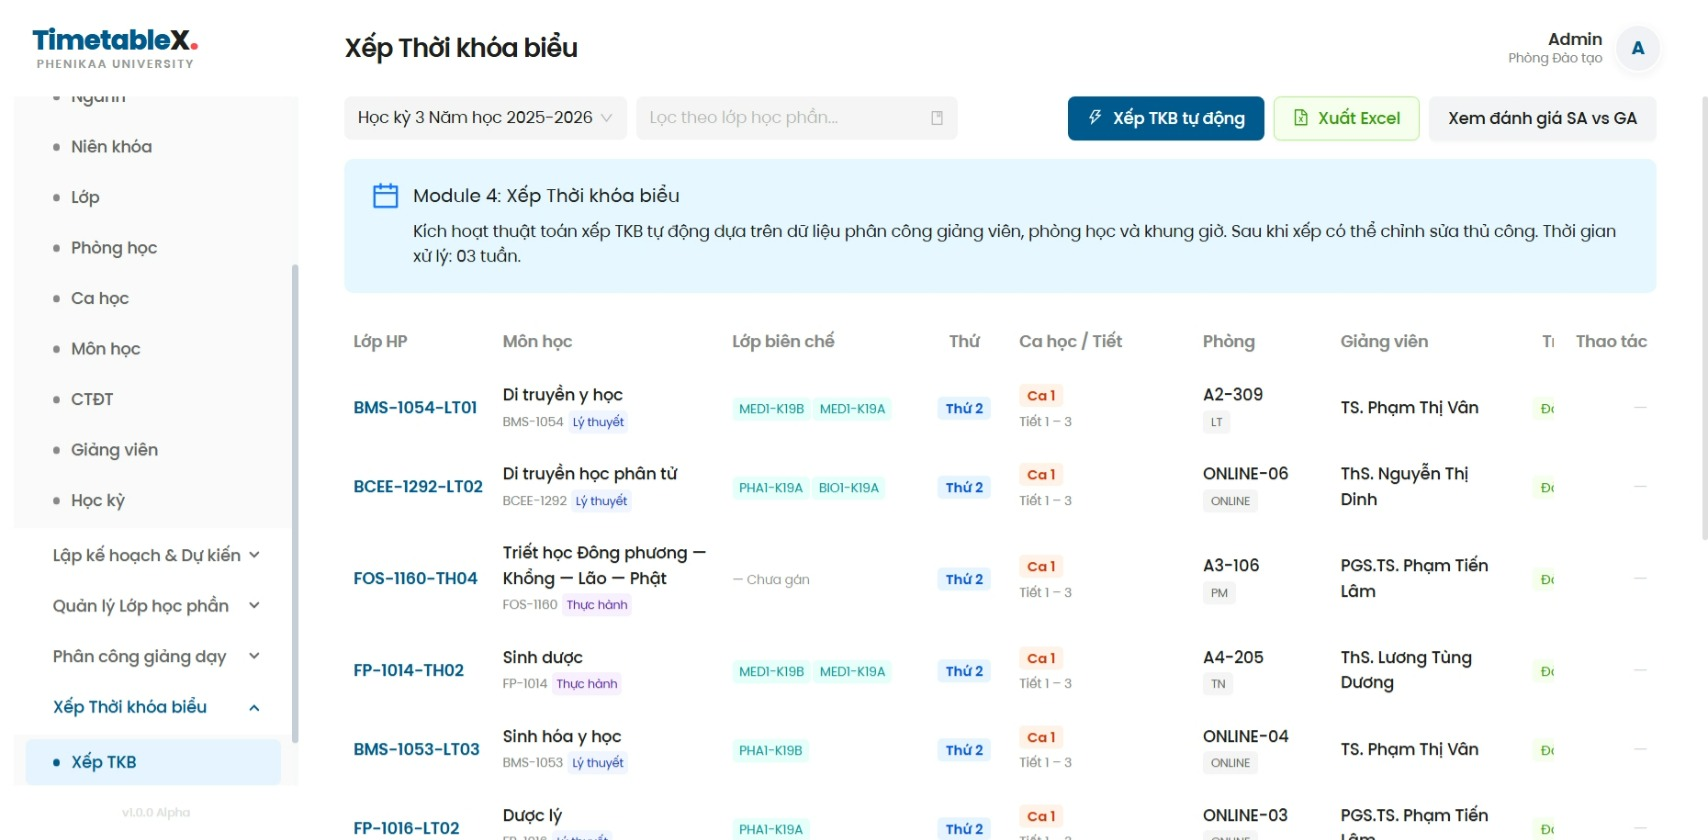
\includegraphics[width=0.48\linewidth]{assets/Screenshot_6-4-2026_173932_localhost.jpeg}
					\hfill
					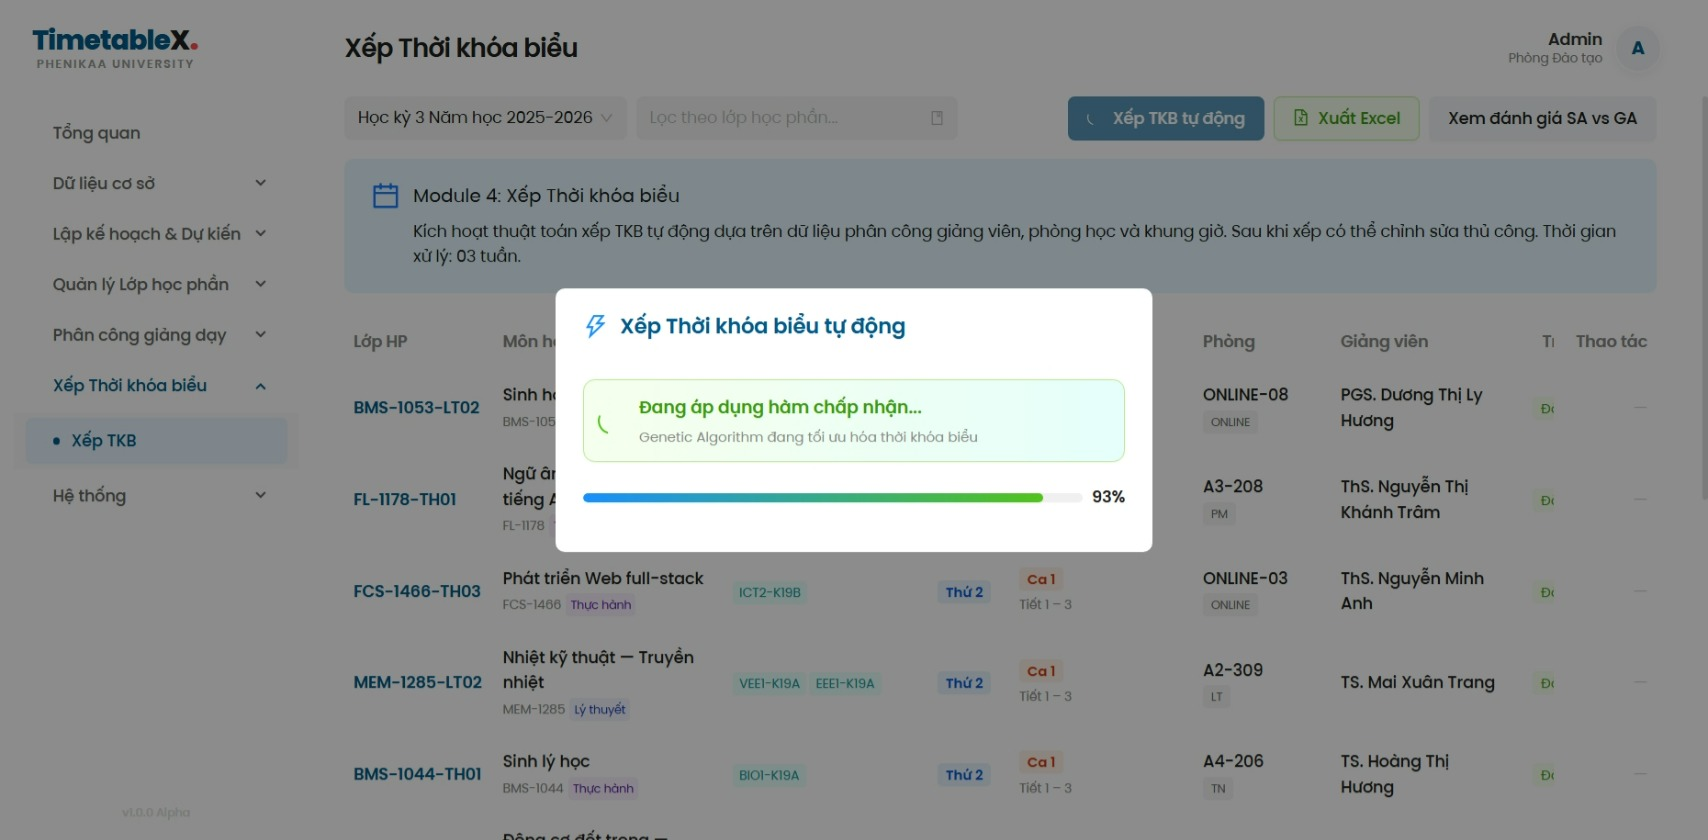
\includegraphics[width=0.48\linewidth]{assets/Screenshot_6-4-2026_192841_localhost.jpeg}
					
					\vspace{0.4cm}
					\normalsize \textit{Hình 1: Giao diện web hệ thống Quản lý và Tự động sinh TKB ứng dụng công nghệ lõi GA.}
					\vspace{0.2cm}
				}
			}
			
			\block{6. Thảo luận}{
				Dựa trên quan trắc chuyên sâu thực tế:
				\begin{itemize}[label=$\blacktriangleright$, itemsep=0.3cm]
					\item \textbf{Phá vỡ tối ưu cục bộ (Anti-Local-Optima)}: Nhờ duy trì biến thể dị hợp ở kích thước 220 cá thể, GA dễ dàng thoát khỏi hiện tượng kẹt cực tiểu mà thuật toán SA đơn nghiệm thường gặp.
					\item \textbf{Tối ưu hóa thời khóa biểu}: GA có độ nhạy tuyệt đối với các hàm mục tiêu phụ, chủ động điều chỉnh để tránh xếp các ca học vào buổi tối muộn, hạn chế tình trạng lịch học bị dàn trải sang ngày cuối tuần.
				\end{itemize}
			}
			
			\block{7. Kết luận}{
				Kết quả nghiên cứu thực nghiệm đã minh họa tính đúng đắn và hiệu suất tối đa của Thuật toán Di truyền (GA) ứng dụng vào bài toán UCTP hiện hành. Kiến trúc này hỗ trợ tự động tính toán khối lượng dữ liệu đồ sộ, triệt tiêu lỗi chủ quan và tự động hóa tối đa quá trình phân bổ tài nguyên giáo dục. Kiến trúc phần mềm hoàn toàn đáp ứng khả năng tích hợp thực tế tại hệ thống điện toán của trường.
			}
			
			
		\end{columns}
		
	\end{document}
